\subsection{Analiza z GeoGebro}

\subsubsection{Sledovi (traces in loci)}

Sledovi (ang. \textit{traces}) in loci (ang. \textit{loci}) so uporabna orodja v GeoGebri za analizo geometrijskih in funkcijskih lastnosti. Sledovi omogočajo sledenje poti točke, ki se premika glede na druge objekte, medtem ko loci prikazujejo množico točk, ki izpolnjujejo določene pogoje.
Razlika med sledovi in loci je v tem, da sledovi prikazujejo pot posamezne točke, medtem ko loci prikazujejo celotno množico točk, ki izpolnjujejo določene pogoje. Najlaže je, da to ponazorimo z naslednjo konstrukcijo:

\begin{framed}
\textbf{Glej tudi}\\
Peucellier-Lipkinov mehanizem je opisan tudi na \href{https://en.wikipedia.org/wiki/Peaucellier\%E2\%80\%93Lipkin\_linkage}{Wikipediji} (ang.). To je mehanizem, ki pretvarja krožno gibanje v ravno linijsko gibanje. Uporablja se lahko za risanje ravnih črt brez uporabe ravnila, poleg tega, lahko tudi uporabimo za risanje krožnic brez uporabe kompasa.
\end{framed}

Lahko tudi uporabimo orodja 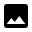
\includegraphics[width=0.0275\linewidth]{files/32px-Mode_image.svg-4ad09c46e3d21949ce372e4d0648d1bc.png}

 \textit{Image} (\textit{Slika}) za uvoz slike mačke in nato sledimo poti določene točke na sliki. To je prikazano v naslednjem konstrukciji:

Če želite, lahko to konstrukcijo odprete v GeoGebri \href{https://www.geogebra.org/classic/hmycsecx}{tukaj}. \textbf{Poskusite sami!}, Če želite, lahko uporabite moje slike: \href{/wall-2f1cf445f820b17acd3ef1477ed55808.png}{wall.png} in \href{/cat-047eeea8d3ff40424daab3c0f825a5f0.png}{cat.png}.

\subsubsection{Funkcije}

GeoGebra ima veliko vnaprerej določenih funkcij, ki jih lahko uporabimo za analizo. Nekatere izmed teh funkcij vključujejo: \texttt{sin()} (sinus), \texttt{cos()} (kosinus), \texttt{tan()} (tangens), \texttt{exp()} (eksponentna funkcija), \texttt{ln()} (naravni logaritem) in še več. (celoten seznam (v ang.) \href{https://geogebra.github.io/docs/manual/en/Predefined\_Functions\_and\_Operators/}{tukaj}) Te funkcije lahko uporabimo za ustvarjanje grafov in izvajanje različnih analiz.

Za uporaba funkcije v GeoGebri, preprosto vnesite ime funkcije, sledeno z oklepaji, ki vsebujejo argumente funkcije. Na primer, za risanje grafa funkcije $f(x) = \sin(x)$, vnesite \texttt{f(x) = sin(x)} v vhodno vrstico in pritisnite .

Lahko tudi ustvarimo funkcije, ki so odvisne od drugih objektov v GeoGebri. Na primer, z ukazom \texttt{g(x) = ax\^3 + bx\^2 + cx + d} lahko ustvarimo funkcijo, ki je odvisna od spremenljivk \texttt{a}, \texttt{b},\texttt{c} in \texttt{d}. Te spremenljivke lahko nato nastavimo na določene vrednosti ali jih povežemo z drsniki za dinamično prilagajanje funkcije.

Nekatera pomembna orodja za delo s funkcijami so:

\begin{itemize}
\item Ukaz \texttt{Roots(\textless funkcija\textgreater , \textless min x\textgreater , \textless max x\textgreater  )} najde ničle funkcije na intervalu $[\min x, \max x]$.
\item Ukaz \texttt{Max(\textless funkcija\textgreater , \textless min x\textgreater , \textless max x\textgreater )} najde maksimum funkcije na določenem intervalu.
\item Ukaz \texttt{Min(\textless funkcija\textgreater ,\textless min x\textgreater , \textless max x\textgreater )} najde minimum funkcije na intervalu $[\min x, \max x]$.
\end{itemize}

Če hitro želimo najti nekatere lastnosti funkcije, lahko uporabimo orodje 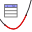
\includegraphics[width=0.0275\linewidth]{files/32px-Mode_functionin-5eeb13f1a6b97d3950fb00eba6b0d8dc.png}

 \textit{Function Inspector} (\textit{Lastnosti funkcije}). To orodje nam omogoča hitro analizo funkcije in izračun njenih lastnosti, kot so ničle, ekstremi, infleksijske točke in še več.

Ko delamo s funkcijami v LaTeXu, je lahko koristno, da uredimo funkcije, s katerimi delamo. Za to, lahko uporabimo orodja 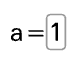
\includegraphics[width=0.0275\linewidth]{files/input-1126993cec2deafac9e4387fbf62c0c6.png}

 \textit{Input box} (\textit{Vhodno polje}). Ko ustvarimo vhodno polje, dobimo okno kjer določamo objekt, ki ga želimo prikazati in urejati \textit{Linked Object} (\textit{Povezani objekt}) in \textit{Caption} (\textit{Naslov}), ki bo prikazan poleg vhodnega polja.

\subsubsection{Odvodi in integrali}

\subsubsection{Polarni krivulje}

GeoGebra omogoča tudi risanje in analizo polarnih krivulj. Polarne krivulje so definirane z enačbami v polarnih koordinatah, kjer je vsaka točka določena z razdaljo od izhodišča (polmer) in kotom glede na pozitivno smer osi $x$.

Poleg tega, lahko prikažemo polarno omrežje v grafičnem oknu z klikom na 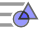
\includegraphics[width=0.0275\linewidth]{files/40px-Stylingbar_icon-dbbb2f8b79b58bbc677f198035a192ed.png}

 \textit{Vrstica za zamenjavo sloga}, nato na 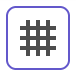
\includegraphics[width=0.0275\linewidth]{files/network-bc241b4229fc5aeeee9f8a77efbc8d93.png}

 \textit{Show grid} (\textit{Omrežje}) in izberemo možnost 
\includegraphics[width=0.0275\linewidth]{files/polarnetwork-e67d0ef442577a3ded203720da15d499.png}

\textit{Polar Grid} (\textit{Polarno omrežje}).

\subsubsection{Parametrične krivulje}

Polarne krivulje so posebna vrsta parametričnih krivulj, kjer je polmer funkcija kota. Vendar pa lahko ustvarimo tudi splošne parametrične krivulje v GeoGebri z uporabo ukaza \texttt{Curve}. Ta ukaz omogoča definiranje krivulje z uporabo dveh funkcij, ki določata $x$ in $y$ koordinate glede na parameter $t$. Na primer, ukaz \texttt{Curve((cos(t), sin(t)), t, 0, 2*$\pi$)} ustvari enoto krožnico.

%  :::{exercise}
% :label: ex-paramentric
% 
% Ustvarite datoteko GeoGebra, ki prikazuje parametrično krivuljo.
% 
% 1. Ustvarite spremenljivki `max_t` in `min_t`.
% 2. Ustvarite funkciji za $x(t)$ in $y(t)$.
% 3. Ustvarite vhodno polje za `max_t` in `min_t`, da lahko spreminjate interval parametra $t$.
% :::

%  ```{margin}
% [Seznam vaj](_vaje)
% ```
% 
% :::{solution} ex-label
% :class: tip dropdown
% :::

%  ```{margin}
% [Seznam vaj](#vaje_geogebraAnaliza)
% ```
% 
% :::{solution} ex-polarni
% :class: tip dropdown
% :::

\subsubsection{Vaje}\label{vaje_geogebraAnaliza}

\begin{itemize}
\item Exercise~\ref{ex-peaucellier} Ustvarite Peaucellier-Lipkinov mehanizem v GeoGebri in analizirajte sled točke $F$.
\item Exercise~\ref{ex-cat} Kako se premika mačka, ko se lestev zdrsne po tleh?
\item Exercise~\ref{ex-functions-1} Ustvarite funkcijo in analizirajte njene lastnosti z orodji GeoGebre.
\item Exercise~\ref{ex-odvod-def} Ustvarite konstrukcijo v GeoGebri, ki omogoča prikaz definicije odvoda funkcije.
\item Exercise~\ref{ex-odvod} V konstrukciji iz prejšnje vaje, dodajte možnost za prikaz grafa odvoda funkcije.
\item Exercise~\ref{ex-integral} Ustvarite konstrukcijo v GeoGebri, ki omogoča prikaz določenega integrala funkcije med točkama $a$ in $b$.
\item Exercise~\ref{ex-polarni} Ustvarite polarne krivulje in analizirajte njihove lastnosti z orodji GeoGebre.
\end{itemize}